\documentclass[../main.tex]{subfiles}

\begin{document}

\begin{enumerate}[a)]
    \item Para pasar de un gráfico $e-T$ a uno $w_\text{tot}- T$ usamos la expresión
\begin{equation}
    w = \frac{e\,\epsilon}{P - e} \simeq \frac{e\epsilon}{P} \label{we}
.\end{equation}

Con esto ya nos hacemos la idea que en el gráfico $w_{tot} - T$, las curvas $w_\text{sat}$ se verán muy similares a la curva $e_\text{sat}$ en el gráfico $e - T$, pero multiplicado por el factor $\dfrac{\epsilon}{P}$. 

    Las curvas para de $w_\text{sat}$ estarán definidas por 
\begin{equation}
    w_\text{sat} = \frac{\epsilon}{P}\,e_\text{sat}(T) \label{wsat}
,\end{equation}
donde $e_\text{sat}(T)$ está dado por la ecuación de Clausius-Clapeyron. Luego, estas se verían como en la figura a continuación 
\begin{figure}[h]
    \centering
            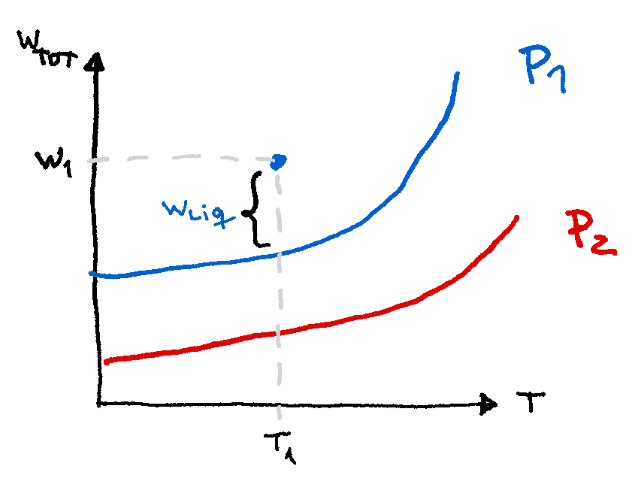
\includegraphics[width=0.6\textwidth]{img/f1}
            \captionof{figure}{Curvas $w_\text{sat}$ para distintas presiones, en función de la temperatura.}
            \label{wsat_p1_p2}
        \end{figure}
En la \autoref{wsat_p1_p2}, la línea azul corresponde a $w_\text{sat}$ a presión $P_1$, mientras que la línea roja corresponde a $w_\text{sat}$ a presión $P_2$, todo esto, con $P_1 < P_2$. Notemos que como en la \autoref{wsat} se divide por $P$, la curva de $w_\text{sat}$ de $P_1$ resulta más grande la de $P_2$.\\

A priori, ubicar un punto (una parcela de aire) en el gráfico $w_\text{tot} - T$ no nos proporciona información para identificar su presión, ya que al incorporar el agua liquida no tenemos una ecuación que relacione $w_\text{tot}$ con la presión. Sin embargo, si ya sabemos su presión de un a parcela, podemos obtener la curva $w_\text{sat}$ a esa presión. 

Si consideramos un punto por debajo de la curva $w_\text{sat}$ (acorde a la presión de la parcela), usando la \autoref{we} obtendremos que ese punto representa una parcela de aire con una presión de vapor $e$ subsaturada $(e < e_\text{sat})$. A medida que ese punto sube (a $T$ constante), inferimos que $e$ se acerca a $e_\text{sat}$, y que $e = e_\text{sat}$ si $w_\text{tot} = w_\text{sat}$, por la \autoref{wsat}. Ahora, si un punto está por sobre la curva $w_\text{sat}$ la \autoref{we} ya no nos sirve, pues esta nos diría que la parcela presenta una presión de vapor superior a $e_\text{sat}$, lo cual no es posible. Dado esto, concluimos que si el punto se encuentra sobre la curva $w_\text{sat}$, la parcela presenta agua liquida. La cantidad de agua liquida corresponderá a la porción de $w_\text{tot}$ que sobresale respecto a la curva. 

En la \autoref{wsat_p1_p2} indicamos que segmento equivale a $w_\text{liq}$, considerando que el punto presenta una parcela de aire con presión $P_1$. Si la parcela tuviese presión $P_2$, $w_\text{liq}$ sería la distancia vertical entre el punto y la curva roja.

\item 
    \begin{enumerate}[\text{Proceso} A:]
        \item Al calentarse la parcela de aire, aumenta su temperatura. Por simplicidad asumimos que $w_\text{tot}$ se mantiene constante, de modo que solo el agua liquida se transforma en vapor.\par
            \begin{minipage}{\linewidth}
                \centering
                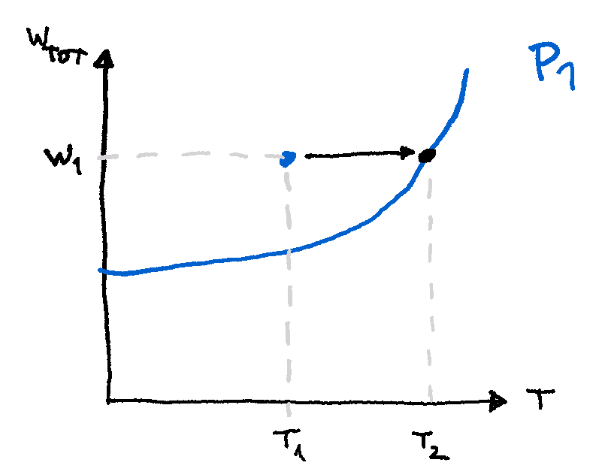
\includegraphics[width=0.6\textwidth]{img/procesoA}
                \captionof{figure}{Proceso A. La flecha negra representa el proceso.}
                \label{fig:pA}
            \end{minipage}\\

            En la \autoref{fig:pA} podemos ver el proceso A. Como la presión es constante, la curva $w_\text{sat}$ no cambia. Luego, el aumento de temperatura hace que el punto ``toque'' a la curva $w_\text{sat}$, siendo ente el momento (punto negro) en que pierde toda su agua líquida.
            \newpage
        \item Como el proceso consiste en precipitación, lo que disminuye es  $w_\text{liq}$.\par
            \begin{minipage}{\linewidth}
                \centering  
                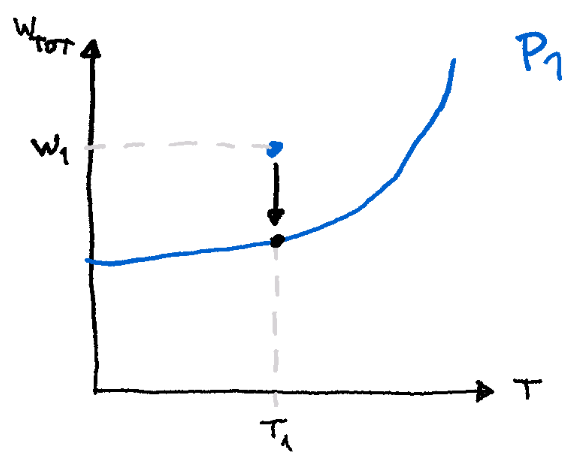
\includegraphics[width=0.6\textwidth]{img/procesoB}
                \captionof{figure}{Proceso B. La flecha negra representa el proceso.}
                \label{pB}
            \end{minipage}\\

            En la \autoref{pB} vemos el proceso B. Como la presión es constante la curva $w_\text{sat}$ no cambia. Como además la temperatura también es constante, no queda otra que $w_\text{tot}$ disminuya. 
        \item En este proceso, como la parcela desciende, la presión cambia (aumenta) , por lo que la curva $w_\text{sat}$ varia (baja). Además, como la parcela tiene agua, esta desciende siguiendo un proceso pseudo-adiabático, implicando que a medida que desciende la temperatura aumenta.\par
\begin{minipage}{\linewidth}
    \centering
    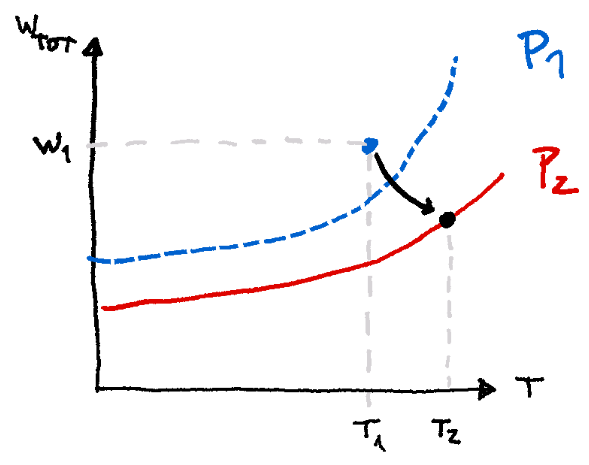
\includegraphics[width=0.6\textwidth]{img/procesoC}
    \captionof{figure}{Proceso C. La flecha negra representa el proceso. La linea segmentada azul representa la curva $w_\text{sat}$ inicial, mientras que la linea roja representa la curva $w_\text{sat}$ final.}
    \label{fig:pC}
\end{minipage}\\

    Considero que acá $w_\text{tot}$ disminuye porque según la \autoref{we}, si la presión aumenta, $w_\text{vap}$ disminuye
    \newpage
    \item Para la mezcla de dos parcelas consideraremos lo siguiente.

        Primero, veamos la relación entre la humedad específica
        $$q = \frac{m_\text{w}}{m_\text{w} + m_\text{a} }$$
       y la razón de mezcla
    $$w = \frac{m_\text{w}}{m_\text{a}}  $$
    con $m_\text{a}$ la masa de aire en la parcela, y $m_\text{w}$ la masa de agua en la parcela.

    Notemos que se cumple 
    \begin{equation}
        \frac{1}{q} = \frac{1}{w} + 1 \label{qw}
    \end{equation}
    Ahora, consideraremos que las dos parcelas que se combinan tienen una masa similar o equivalente. 
    Por ejemplo, diremos que la parcela 1 presenta una masa $m = m_\text{v}+ m_\text{l} + m_\text{a}$ (con $m_\text{v}$ la masa del agua en forma de vapor, $m_\text{l}$ la masa de agua en forma líquida, y $m_\text{a}$ la masa del aire), y que la parcela 2, que es solo aire (ya que está completamente seca), también tiene una masa $m$.\\

    Con esto ya podemos calcular la humedad específica de la parcela mezclada. Esta parcela debiese tener masa $2m$ por lo que su humedad específica será
    \begin{equation}
        q_\text{mezcla} = \frac{m_\text{w}}{2m} = \frac{m_\text{w}}{2(m_\text{w} + m_\text{a})}
    \end{equation}
con $m_\text{w} = m_\text{l} + m_\text{v}$. Luego, usando la \autoref{qw}, obtenemos que la razón de mezcla de la parcela mezclada es 
\begin{equation}
    w_\text{mezcla} = \left[2\, \frac{m_\text{w} + m_\text{a}}{m_\text{w}} -1 \right]^{-1} = \frac{m_\text{w}}{m_w + 2m_\text{a}}
\end{equation}
Calculemos ahora la razón $\frac{w}{w_\text{mezcla}}$, para ver en cuanto disminuye la razón de mezcla luego de mezclarse.
\begin{equation}
    \frac{w}{w_\text{mezcla}} = \frac{\dfrac{m_\text{w}}{m_\text{a}}}{\dfrac{m_\text{w}}{m_\text{w}+2m_\text{a}}} = \frac{m_\text{w} + 2m_\text{a}}{m_\text{a}} = 2 + \frac{m_\text{w}}{m_\text{a}}= 2+ w
\end{equation}
Con esto último podemos decir que 
\begin{equation}
    w_\text{mezcla} = \frac{w}{2+w}
\end{equation}
Es decir, prácticamente la razón de mezcla se reduce a un poco menos de la mitad del valor inicial.\\

Para que luego de este proceso, la parcele quede sin agua liquida necesitamos que $w_\text{mezcla}$ resulte menor o igual que $w_\text{sat}$. Desarrollando esta desigualdad obtenemos lo siguiente:
\begin{align*}
    \frac{w}{w+2} &\le w_\text{sat}\\
    w &\le  w_\text{sat}(2 + w)\\
    w &\le 2w_\text{sat} ww_\text{sat}\\
    w(1-w_\text{sat}) &\le 2w_\text{sat}\\
    w &\le \frac{2}{1-w_\text{sat}} w_\text{sat}\\
    w_\text{l} + w_\text{v} &\le \frac{2}{1-w_\text{sat}} w_\text{sat}
.\end{align*}
Como sabemos que  $w_\text{v}$ (parte en vapor) si o sí es menor o igual que $w_\text{sat}$ obtenemos
    \begin{align*}
    w_\text{l} &\le \frac{2}{1-w_\text{sat}} w_\text{sat} - w_\text{sat}\\
    w_\text{l} &\le \frac{w_\text{sat}}{1- w_\text{sat}} + \frac{w_\text{sat}^2}{1-w_\text{sat}}
    .\end{align*}

Entonces, solo si se cumple esta condición en la parcela de aire inicial, la parcela final queda sin agua líquida. Para simplificar la condición anterior podemos despreciar $w_\text{sat}^2$ por ser muy pequeño, y si además consideramos $w_\text{sat}\ll 1$, nos queda que $w_\text{l} \le w_\text{sat}$. Es decir, aproximadamente la porción líquida de la razón de mezcla debe ser menor al valor de $w_\text{sat}$ para la presión y temperatura de la parcela.\par
\begin{minipage}{\linewidth}
    \centering
    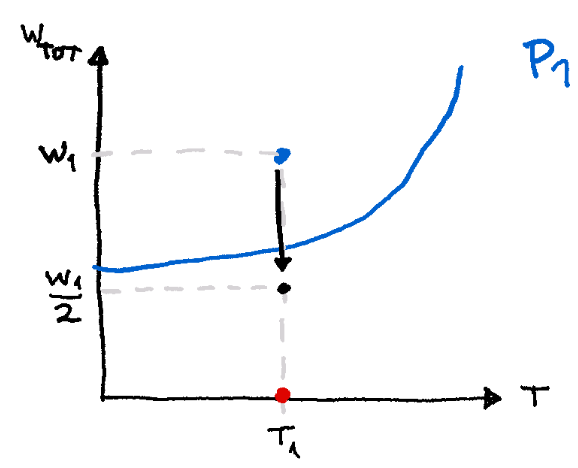
\includegraphics[width=0.6\textwidth]{img/procesoD}
    \captionof{figure}{Proceso D. La flecha negra representa el proceso. El punto azul corresponde a la parcela con agua mientras que el punto rojo corresponde a la parcela seca. Luego el punto negro corresponde aproximadamente a la mezcla entre las dos parcelas iniciales.}
    \label{fig:pD}
    
\end{minipage}

    \end{enumerate}

\end{enumerate}



\end{document}
